% Provenance (never printed): enseignement scientifique premiere (2019),
% "La Terre, un astre singulier" (the place of the Earth) and the old seconde
% SVT "La planete Terre, une planete habitable" (conditions for liquid water,
% the habitable zone); see sources/book2/PROVENANCE.md. Every temperature,
% phase boundary and habitable-zone limit is computed in
% figdata/grade-10/planet_temperatures.py.
\chapter{Um planeta habitável}\label{ch:g10:habitable-planet}

Três planetas rochosos giram lado a lado em torno do Sol. Na superfície de
Vênus, o ar é tão denso que pressiona noventa e duas vezes mais que na
Terra, e tão quente --- mais de \qty{460}{\degreeCelsius} --- que o chumbo
derreteria. Em Marte, o ar rarefeito pressiona menos de um centésimo do que
o nosso, e a temperatura média fica muito abaixo do ponto de congelamento.
Entre os dois, a Terra tem oceanos, chuva e vida. Os três planetas se
formaram do mesmo disco de gás e poeira em torno do jovem Sol, a partir
praticamente das mesmas rochas. Por que destinos tão diferentes? Este
capítulo examina o que fixa a temperatura de um planeta, o que lhe permite
conservar uma atmosfera, em que condições a água pode ser líquida e onde,
em torno do Sol e de outras estrelas, essas condições podem ser
encontradas.
% ledger: nasa:venus-atm, nasa:mars-atm, planet:Venus.Tmean

\begin{omfigure}
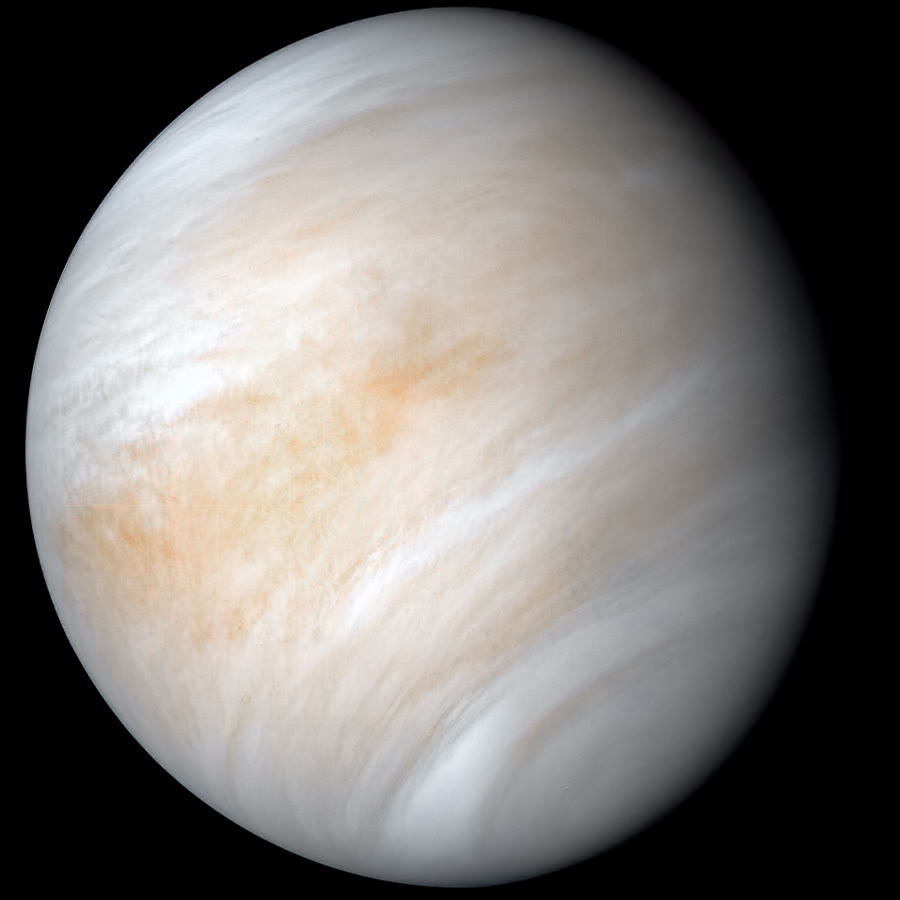
\includegraphics[width=0.38\linewidth]{images/book2/g10-nasa-venus-mariner10.jpg}

{\small Vênus vista pela sonda Mariner~10 em 1974, em cores próximas das que
o olho veria: um planeta inteiramente envolto em nuvens. Imagem:
NASA/JPL-Caltech (domínio público).}
\end{omfigure}

\begin{recall}
O Sol é uma estrela; em torno dele, os quatro planetas rochosos, Mercúrio,
Vênus, a Terra e Marte, e depois os quatro planetas gigantes, percorrem
órbitas quase circulares (os livros de física e o Livro 1). Todo corpo
irradia energia na forma de luz, tanto mais quanto mais alta for a sua
temperatura, sobretudo como luz infravermelha nas temperaturas dos
planetas (os livros de física). Os gases de efeito estufa --- vapor de
água, gás carbônico, metano --- absorvem parte do infravermelho emitido por
uma superfície e a mantêm mais quente (os livros de química). A água existe
como gelo, água líquida e vapor de água; a pressão é uma força por unidade
de área, medida em pascals (os livros de física).
\end{recall}

\section{A temperatura fixada pela estrela}

O Sol envia a sua luz igualmente em todas as direções. A uma distância $d$,
a sua potência $L$ (a sua \emph{luminosidade}) se espalha sobre uma esfera
de área $4\pi d^2$.

\begin{proposition}[A lei do inverso do quadrado da luz solar]\label{prop:g10:habitable-planet:inverse-square}
A potência recebida por metro quadrado voltado para o Sol, a
\emph{irradiância solar}, a uma distância $d$ do Sol é
\[
  S = \frac{L}{4\pi d^2}.
\]
À distância da Terra, \qty{1}{au}, $S_0 = \qty{1361}{W/m^2}$; a uma
distância $d$ medida em unidades astronômicas, $S = S_0/d^2$.
\end{proposition}

\begin{proof}
Nenhuma luz se perde no espaço vazio, logo toda a potência $L$ atravessa
cada esfera centrada no Sol; numa esfera de raio $d$, ela se reparte por
$4\pi d^2$ metros quadrados. Dobrar $d$ multiplica a área por quatro e
divide $S$ por quatro.
\end{proof}
% ledger: earth:TSI, sun:L, const:au

\begin{omfigure}
\begin{tikzpicture}[font=\small, >={Stealth[length=2mm]}]
  \shade[ball color=yellow!70!orange] (0,0) circle (0.35);
  \node[below=4pt] at (0,-0.35) {Sol};
  \draw[omThm!70, thick] (0,0) -- (3,0.6) (0,0) -- (3,-0.6);
  \draw[omThm!70, thick, dashed] (3,0.6) -- (6,1.2) (3,-0.6) -- (6,-1.2);
  \draw[fill=omDef!25, draw=omDef!80!black] (3,-0.6) rectangle (3.18,0.6);
  \draw[fill=omDef!12, draw=omDef!80!black] (6,-1.2) rectangle (6.18,1.2);
  \draw[omDef!80!black] (6,0) -- (6.18,0) (6.09,-1.2) -- (6.09,1.2);
  \node[anchor=north] at (3.1,-0.7) {$d$};
  \node[anchor=north] at (6.1,-1.3) {$2d$};
  \node[anchor=south east, align=right, font=\footnotesize] at (2.9,0.75) {1 quadrado:\\toda a luz};
  \node[anchor=west, align=left, font=\footnotesize] at (6.35,0.6) {4 quadrados:\\um quarto cada};
  \draw[->, black!60] (0.5,-1.95) -- (6.1,-1.95);
  \node[anchor=north, font=\footnotesize] at (3.3,-2.0) {distância ao Sol};
\end{tikzpicture}

{\small A luz que atravessa um quadrado à distância $d$ se espalha por
quatro quadrados do mesmo tamanho à distância $2d$: a irradiância diminui
como o inverso do quadrado da distância.}
\end{omfigure}

Um planeta absorve a parte dessa luz que ele não reflete e irradia energia
para o espaço na forma de luz infravermelha. Se absorve mais do que irradia,
ele se aquece; mais quente, irradia mais; e se estabiliza na temperatura em
que as duas se equilibram.

\begin{definition}[Temperatura de equilíbrio]\label{def:g10:habitable-planet:equilibrium-temperature}
A \emph{temperatura de equilíbrio}\index{temperatura de equilibrio@temperatura de equilíbrio}
de um planeta é a temperatura em que um corpo que irradiasse como um
emissor perfeito enviaria para o espaço exatamente a potência que o planeta
absorve da sua estrela. A fração da luz incidente que o planeta, como um
todo, reflete é o seu \emph{albedo de Bond} $A$.
\end{definition}

\begin{proposition}[Cálculo da temperatura de equilíbrio]\label{prop:g10:habitable-planet:teq}
Para um planeta que distribui o calor absorvido por toda a sua superfície,
\[
  T_{\mathrm{eq}} = \left(\frac{S\,(1-A)}{4\sigma}\right)^{1/4},
  \qquad \sigma = \qty{5.67e-8}{W.m^{-2}.K^{-4}}.
\]
À distância da Terra e sem nenhuma reflexão, isso dá \qty{278.3}{K}; a uma
distância $d$ em unidades astronômicas e com albedo $A$,
$T_{\mathrm{eq}} = \qty{278.3}{K} \times (1-A)^{1/4}/\sqrt{d}$.
\end{proposition}

\begin{proof}[Demonstração parcial]
O planeta intercepta a luz do Sol num disco de área $\pi R^2$ e absorve a
potência $(1-A)\,S\,\pi R^2$. Ele irradia por toda a sua superfície,
$4\pi R^2$. Um emissor perfeito à temperatura $T$ irradia $\sigma T^4$ por
metro quadrado (uma lei demonstrada nos livros de física e admitida aqui).
Igualar $4\pi R^2 \sigma T^4 = (1-A)\,S\,\pi R^2$ dá a fórmula; o raio se
cancela. Com $S = S_0/d^2$, a raiz quarta de $1/d^2$ é $1/\sqrt d$.
\end{proof}
% ledger: const:sigma, earth:TSI

\begin{example}[A Terra]\label{ex:g10:habitable-planet:earth}
% ledger: earth:TSI, earth:albedo, earth:Tbb, earth:Tsurf
Com $S_0 = \qty{1361}{W/m^2}$ e $A = 0.294$,
$T_{\mathrm{eq}} = 278.3 \times 0.706^{1/4} \approx \qty{255}{K}$, isto é,
\qty{-18}{\degreeCelsius}. (A ficha técnica da NASA indica \qty{254}{K}.) A
temperatura média da superfície da Terra é de \qty{288}{K},
\qty{15}{\degreeCelsius}: o efeito estufa da atmosfera a aquece em cerca de
\qty{33}{K}. Sem ele, os oceanos congelariam.
\end{example}

\begin{omfigure}
\begin{tikzpicture}
\begin{axis}[ybar, width=0.86\linewidth, height=5.8cm, ymin=0, ymax=950,
  bar width=10pt, enlarge x limits=0.15, symbolic x coords={Mercury,Venus,Earth,Moon,Mars},
  xtick=data, xticklabels={Mercúrio,Vênus,Terra,Lua,Marte}, ylabel={temperatura (K)}, ymajorgrids, grid style={gray!22},
  legend style={at={(0.97,0.95)}, anchor=north east, font=\footnotesize, draw=black!30},
  nodes near coords, nodes near coords style={font=\scriptsize, rotate=90, anchor=west, /pgf/number format/fixed, /pgf/number format/precision=0},
  tick label style={font=\small}, label style={font=\small}]
\addplot[fill=omDef!45, draw=omDef!80!black] table[x=name, y=Teq_K] {figdata/out/grade-10-planet_temperatures-planets.dat};
\addlegendentry{temperatura de equilíbrio}
\addplot[fill=omThm!55, draw=omThm!80!black] table[x=name, y=Tmean_K] {figdata/out/grade-10-planet_temperatures-planets.dat};
\addlegendentry{temperatura média medida da superfície}
\end{axis}
\end{tikzpicture}

{\small \omterm{def:g10:habitable-planet:equilibrium-temperature}{Temperaturas de equilíbrio} calculadas a partir da distância e do
albedo de Bond de cada corpo, ao lado das temperaturas médias medidas das
suas superfícies. Dados: fichas planetárias da NASA.}
\end{omfigure}

\begin{remark}[Leitura do gráfico]\label{rem:g10:habitable-planet:reading}
% ledger: nasa:bond-albedos, planet:Mercury.Tmean, planet:Venus.Tmean, planet:Moon.Tmean, planet:Mars.Tmean, planet:Moon.day, nasa:moon-temps
Para Mercúrio e Marte, que quase não têm atmosfera ou têm uma muito
rarefeita, a média medida fica perto da \omterm{def:g10:habitable-planet:equilibrium-temperature}{temperatura de equilíbrio}. A média
da Lua fica abaixo dela: lá, cada dia e cada noite duram cerca de duas
semanas, e a superfície oscila entre cerca de \qty{95}{K} e \qty{390}{K}, o
que a fórmula simples, feita para um planeta que distribui o calor de modo
uniforme, não descreve. Vênus é o caso marcante: com um albedo de Bond de
0.77 --- as suas nuvens refletem a maior parte da luz do Sol ---, a sua
\omterm{def:g10:habitable-planet:equilibrium-temperature}{temperatura de equilíbrio} é mais baixa que a da Terra, e no entanto a sua
superfície é mais de \qty{500}{K} mais quente que isso: é o efeito estufa
da sua espessa atmosfera de gás carbônico.
\end{remark}

\section{Conservar uma atmosfera}

Um gás é feito de moléculas em movimento constante, tanto mais rápidas
quanto mais quente o gás. Uma molécula no topo de uma atmosfera que se move
para cima mais depressa que a velocidade de escape do planeta --- a
velocidade necessária para deixar de vez a sua gravidade (os livros de
física) --- se perde no espaço. Ao longo de bilhões de anos, um planeta
pequeno, de gravidade fraca, perde o seu ar; um grande o conserva.

\begin{center}
\small
% ledger: planet:Mercury.vesc, planet:Venus.vesc, planet:Earth.vesc, planet:Moon.vesc, planet:Mars.vesc, planet:Mercury.psurf, planet:Venus.psurf, planet:Earth.psurf, planet:Moon.psurf, nasa:mars-atm
\begin{tabular}{lccc}
\hline
corpo & velocidade de escape (\unit{km/s}) & pressão na superfície (bar) & atmosfera \\
\hline
Lua & 2.4 & 0 & nenhuma \\
Mercúrio & 4.3 & 0 & nenhuma \\
Marte & 5.0 & 0.006 & rarefeita, gás carbônico \\
Vênus & 10.4 & 92 & espessa, gás carbônico \\
Terra & 11.2 & 1 & nitrogênio e oxigênio \\
\hline
\end{tabular}
\end{center}

\begin{remark}[O tamanho não explica tudo]\label{rem:g10:habitable-planet:size}
A Lua e Mercúrio, pequenos e (no caso de Mercúrio) perto do Sol quente,
perderam quase todos os seus gases. Marte, com a metade da velocidade de
escape da Terra, conservou uma atmosfera rarefeita. Vênus e a Terra têm
quase o mesmo tamanho e a mesma velocidade de escape, e no entanto
atmosferas muito diferentes: as suas histórias --- o destino da sua água e
do seu gás carbônico --- divergiram, como o \cref{ch:g12:early-earth}
mostrará para a Terra.
\end{remark}

\section{A água líquida}

\begin{omfigure}
\begin{tikzpicture}
\begin{axis}[omrecord, width=0.88\linewidth, height=7.2cm, xmin=150, xmax=800,
  ymode=log, ymin=1e-6, ymax=2000, xlabel={temperatura (K)}, ylabel={pressão (bar)},
  xtick={200,300,...,800}, ytick={1e-6,1e-4,1e-2,1,100},
  log basis y=10]
\addplot[omDef!85!black, line width=1.1pt] table[x=T_K, y=p_bar] {figdata/out/grade-10-planet_temperatures-vap.dat};
\addplot[omDef!85!black, line width=1.1pt] table[x=T_K, y=p_bar] {figdata/out/grade-10-planet_temperatures-subl.dat};
\addplot[omDef!85!black, line width=1.1pt] table[x=T_K, y=p_bar] {figdata/out/grade-10-planet_temperatures-melt.dat};
\addplot[only marks, mark=*, mark size=2pt, black] coordinates {(273.16,0.00611657) (647.096,220.64)};
\addplot[only marks, mark=square*, mark size=2.4pt, omThm!85!black] table[x=T_K, y=p_bar] {figdata/out/grade-10-planet_temperatures-points.dat};
\node[font=\small] at (axis cs:205,30) {gelo};
\node[font=\small] at (axis cs:420,30) {líquido};
\node[font=\small] at (axis cs:600,1e-3) {vapor de água};
\node[font=\footnotesize, anchor=north west] at (axis cs:276,0.0055) {ponto triplo};
\node[font=\footnotesize, anchor=south east] at (axis cs:640,300) {ponto crítico};
\node[font=\footnotesize, anchor=south, omThm!85!black] at (axis cs:737,110) {Vênus};
\node[font=\footnotesize, anchor=west, omThm!85!black] at (axis cs:296,1.0) {Terra};
\node[font=\footnotesize, anchor=north, omThm!85!black] at (axis cs:210,0.0045) {Marte};
\end{axis}
\end{tikzpicture}

{\small O diagrama de fases da água, com as condições médias na superfície
de Vênus, da Terra e de Marte (quadrados). O eixo das pressões é
logarítmico: cada marca vale cem vezes a de baixo. Curvas calculadas com as
equações da Associação Internacional para as Propriedades da Água e do
Vapor (IAPWS); valores planetários da NASA.}
\end{omfigure}

\begin{proposition}[Quando a água pode ser líquida]\label{prop:g10:habitable-planet:liquid}
% ledger: iapws:triple-critical, iapws:vapour-pressure, iapws:melt-subl
A água líquida só existe a pressões acima da do \emph{ponto triplo},
\qty{611.657}{Pa} (\qty{0.006}{bar}), em que gelo, líquido e vapor coexistem
a \qty{273.16}{K}, e a temperaturas abaixo do \emph{ponto crítico},
\qty{647.096}{K} (\qty{220.64}{bar}), além do qual líquido e vapor não podem
mais ser distinguidos. A uma pressão dada, acima do ponto triplo, a água é
líquida entre o seu ponto de fusão, perto de \qty{273}{K}, e o seu ponto de
ebulição, que baixa quando a pressão baixa.
\end{proposition}

\begin{example}[Três planetas num só diagrama]\label{ex:g10:habitable-planet:three}
% ledger: nasa:venus-atm, nasa:mars-atm, earth:psurf, earth:Tsurf (boiling point at 636 Pa computed)
A superfície da Terra, a \qty{288}{K} e \qty{1}{bar}, fica dentro do campo
do líquido: ali a água pode ser líquida, gelo ou vapor, conforme o tempo.
Vênus, a \qty{737}{K}, fica muito além da temperatura crítica: nenhuma água
líquida é possível. Marte, a \qty{6.36}{mbar}, fica logo acima do ponto
triplo: ali a água ferve a cerca de \qty{0.5}{\degreeCelsius}, de modo que
a água líquida só poderia sobreviver numa janela de cerca de meio grau, e a
temperatura média, \qty{210}{K}, está no campo do gelo.
\end{example}

\begin{omfigure}
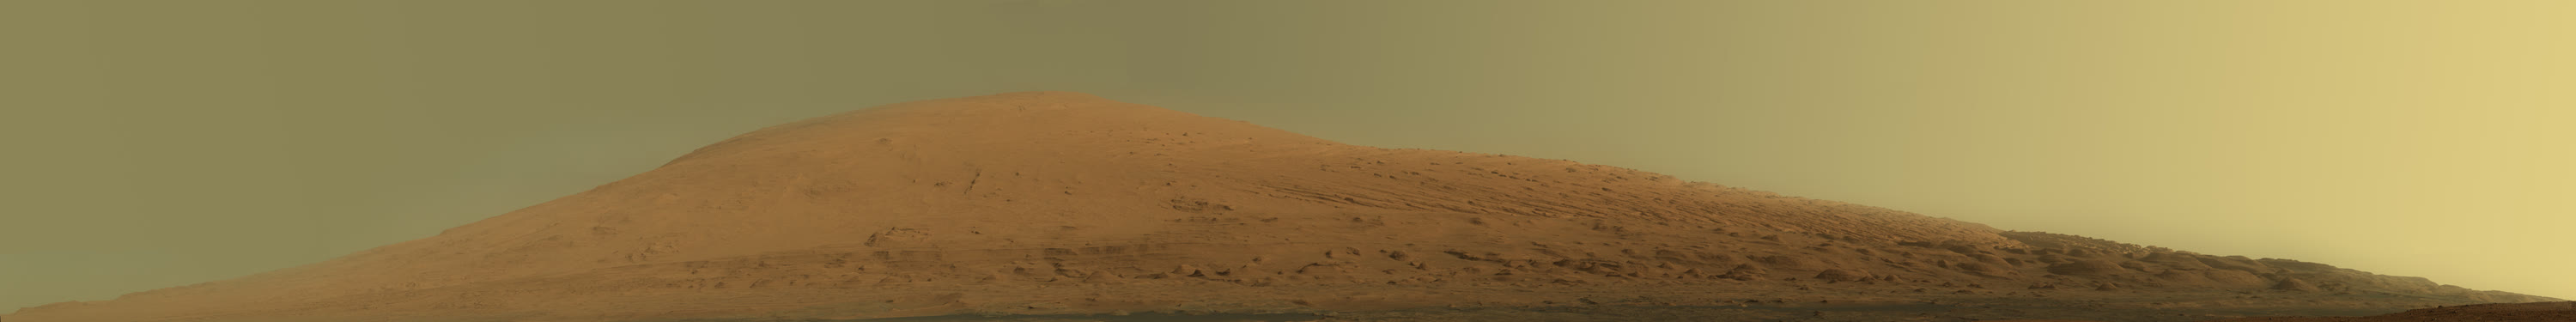
\includegraphics[width=0.96\linewidth]{images/book2/g10-nasa-mars-mount-sharp.jpg}

{\small O monte Sharp, dentro da cratera Gale, em Marte, fotografado pelo
jipe-robô Curiosity em 2012, nas cores registradas pela sua câmera. As suas
camadas inferiores foram depositadas na água, há bilhões de anos. Imagem:
NASA/JPL-Caltech/MSSS (domínio público).}
\end{omfigure}

\section{A zona habitável}

\begin{definition}[Zona habitável]\label{def:g10:habitable-planet:habitable-zone}
A \emph{zona habitável}\index{zona habitavel@zona habitável} de uma estrela
é o intervalo de distâncias à estrela em que um planeta rochoso com água
suficiente e uma atmosfera como a da Terra poderia conservar água líquida
na sua superfície. A sua borda interna fica onde o planeta perderia a sua
água para o calor; a sua borda externa, onde nem mesmo um forte efeito
estufa conseguiria mais impedir que ela congelasse.
\end{definition}

\begin{proposition}[A zona habitável do Sol]\label{prop:g10:habitable-planet:hz-sun}
% ledger: kopparapu:hz-sun, planet:Mercury.dist, planet:Venus.dist, planet:Mars.dist
Modelos detalhados de atmosferas planetárias situam a \omterm{def:g10:habitable-planet:habitable-zone}{zona habitável} do Sol
entre \qty{0.99}{au} e \qty{1.70}{au}. A Terra (\qty{1}{au}) fica logo
dentro da sua borda interna; Marte (\qty{1.52}{au}) fica dentro dela;
Vênus (\qty{0.72}{au}) fica bem aquém da borda interna.
\end{proposition}

\begin{proposition}[Zonas habitáveis de outras estrelas]\label{prop:g10:habitable-planet:hz-scaling}
Em torno de uma estrela de luminosidade $L$, um planeta recebe a mesma
irradiância que a uma distância $d_\odot$ do Sol quando fica a
\[
  d = d_\odot \sqrt{L/L_\odot}.
\]
As bordas da \omterm{def:g10:habitable-planet:habitable-zone}{zona habitável} se deslocam na mesma proporção, numa primeira
aproximação (a cor da luz da estrela também importa um pouco).
\end{proposition}

\begin{proof}
Irradiância igual significa $L/(4\pi d^2) = L_\odot/(4\pi d_\odot^2)$, logo
$d^2 = d_\odot^2\,L/L_\odot$.
\end{proof}

\begin{omfigure}
\begin{tikzpicture}[font=\small]
  % top: the Sun, 0-2 au over 12 cm (6 cm per au)
  \fill[omProp!30] (0.99*6,0) rectangle (1.70*6,0.5);
  \draw[black!70] (0,0.25) -- (12.3,0.25);
  \foreach \x in {0,0.5,...,2} \draw (\x*6,0.15) -- (\x*6,0.35) node[pos=0, below=1pt, font=\footnotesize] {\x};
  \shade[ball color=yellow!70!orange] (0,0.25) circle (0.22);
  \foreach \n/\d in {Mercúrio/0.387, Vênus/0.723, Terra/1.0, Marte/1.524} {
    \fill[omThm!85!black] (\d*6,0.25) circle (2.2pt);
    \node[anchor=south, font=\footnotesize] at (\d*6,0.55) {\n};
  }
  \node[anchor=west, font=\footnotesize] at (12.4,0.25) {au};
  \node[anchor=north, font=\footnotesize] at (8.07,-0.25) {zona habitável, 0.99--1.70 au};
  \node[anchor=east, font=\footnotesize] at (-0.3,0.25) {Sol};
  % bottom: Proxima Centauri, 0-0.1 au over 12 cm (120 cm per au)
  \begin{scope}[yshift=-2.2cm]
  \fill[omProp!30] (0.0385*120,0) rectangle (0.0661*120,0.5);
  \draw[black!70] (0,0.25) -- (12.3,0.25);
  \foreach \x/\l in {0/0, 0.025/0.025, 0.05/0.05, 0.075/0.075, 0.1/0.1} \draw (\x*120,0.15) -- (\x*120,0.35) node[pos=0, below=1pt, font=\footnotesize] {\l};
  \shade[ball color=red!70!orange] (0,0.25) circle (0.14);
  \fill[omThm!85!black] (0.0485*120,0.25) circle (2.2pt);
  \node[anchor=south, font=\footnotesize] at (0.0485*120,0.55) {Proxima b};
  \node[anchor=west, font=\footnotesize] at (12.4,0.25) {au};
  \node[anchor=north, font=\footnotesize] at (6.28,-0.25) {zona habitável, 0.038--0.066 au};
  \node[anchor=east, align=right, font=\footnotesize] at (-0.3,0.25) {Proxima\\Centauri};
  \end{scope}
\end{tikzpicture}

{\small Em cima: a \omterm{def:g10:habitable-planet:habitable-zone}{zona habitável} do Sol e os quatro planetas rochosos. Embaixo:
a \omterm{def:g10:habitable-planet:habitable-zone}{zona habitável} da tênue estrela vermelha Proxima Centauri, calculada
ajustando a do Sol pela raiz quadrada da luminosidade da estrela, e o seu
planeta Proxima~b. Note a mudança de escala: a faixa de baixo inteira mede
\qty{0.1}{au}.}
\end{omfigure}

\section{Planetas de outras estrelas}

\begin{definition}[Exoplaneta]\label{def:g10:habitable-planet:exoplanet}
Um \emph{exoplaneta}\index{exoplaneta} é um planeta que orbita uma estrela
que não é o Sol.
\end{definition}

Os \omterm{def:g10:habitable-planet:exoplanet}{exoplanetas} são fracos demais e próximos demais das suas estrelas para
serem vistos diretamente, com exceção de alguns gigantes. A maioria é
descoberta de forma indireta: ou o planeta passa na frente da sua estrela
uma vez por órbita e a escurece muito levemente, ou a sua atração faz a
estrela oscilar, aproximando-se e afastando-se de nós, o que desloca a cor
da luz da estrela de um lado para o outro. O segundo método dá apenas uma
massa \emph{mínima} para o planeta, porque a inclinação da órbita não é
conhecida. Esses métodos são estudados no volume do terceiro ano da
graduação.

\begin{dated}{2026}
% ledger: nea:count-2026
Em 15 de outubro de 2026, o NASA Exoplanet Archive listava 6\,451
\omterm{def:g10:habitable-planet:exoplanet}{exoplanetas} confirmados.
\end{dated}

\begin{example}[Proxima b]\label{ex:g10:habitable-planet:proxima}
% ledger: nea:proxima-b (flux and habitable zone computed in figdata/grade-10/planet_temperatures.py)
A estrela mais próxima do Sol, Proxima Centauri, a \qty{1.30}{\parsec},
é uma pequena estrela vermelha cuja luminosidade é de apenas cerca de
$0.0015$ da do Sol. Em 2016, foi descoberto um planeta que a orbita a cada
11.2 dias, a \qty{0.0485}{au}, com pelo menos 1.06 vez a massa da Terra. A
essa distância, ele recebe cerca de 0.64 da irradiância que a Terra recebe
e fica dentro da \omterm{def:g10:habitable-planet:habitable-zone}{zona habitável} da sua estrela. Não se sabe se ele tem
atmosfera, nem água.
\end{example}

\begin{remark}[Habitável não quer dizer habitado]\label{rem:g10:habitable-planet:inhabited}
A \omterm{def:g10:habitable-planet:habitable-zone}{zona habitável} diz respeito apenas à distância e à luz. Um planeta dentro
dela pode não ter água, nem atmosfera, ou ter a atmosfera errada --- Marte
fica dentro da zona do Sol e não tem hoje água líquida na sua superfície. A
Terra é habitável porque várias condições valem ao mesmo tempo: a distância
certa, uma massa grande o bastante para conservar uma atmosfera, água em
abundância e um efeito estufa nem fraco nem forte demais.
\end{remark}

\section{Exercícios}

\begin{exercise}[$\star$]\label{exo:g10:habitable-planet:1}
Defina a \omterm{def:g10:habitable-planet:equilibrium-temperature}{temperatura de equilíbrio} de um planeta. Por que a temperatura
média da superfície da Terra é mais alta que a sua \omterm{def:g10:habitable-planet:equilibrium-temperature}{temperatura de equilíbrio}?
\end{exercise}

\begin{exercise}[$\star$]\label{exo:g10:habitable-planet:2}
Usando o gráfico de barras das \omterm{def:g10:habitable-planet:equilibrium-temperature}{temperaturas de equilíbrio} e medidas, indique
o corpo cuja superfície é mais aquecida pela sua atmosfera e estime em
quantos kelvins.
\end{exercise}

\begin{exercise}[$\star$]\label{exo:g10:habitable-planet:3}
Marte orbita a \qty{1.52}{au} do Sol. Usando a lei do inverso do quadrado
com $S_0 = \qty{1361}{W/m^2}$, calcule a irradiância solar em Marte.
\end{exercise}

\begin{exercise}[$\star$]\label{exo:g10:habitable-planet:4}
Usando o diagrama de fases da água, dê o estado da água a \qty{1}{bar} e
\qty{330}{K}; a \qty{0.001}{bar} e \qty{250}{K}; a \qty{100}{bar} e
\qty{700}{K}.
\end{exercise}

\begin{exercise}[$\star$]\label{exo:g10:habitable-planet:5}
O que é um \omterm{def:g10:habitable-planet:exoplanet}{exoplaneta}? Descreva, numa frase cada, as duas principais
maneiras de detectar \omterm{def:g10:habitable-planet:exoplanet}{exoplanetas}.
\end{exercise}

\begin{exercise}[$\star\star$]\label{exo:g10:habitable-planet:6}
Calcule a \omterm{def:g10:habitable-planet:equilibrium-temperature}{temperatura de equilíbrio} da Terra com $S_0 = \qty{1361}{W/m^2}$
e $A = 0.294$ e, depois, com $A = 0$. Converta as duas para graus Celsius.
\end{exercise}

\begin{exercise}[$\star\star$]\label{exo:g10:habitable-planet:7}
Uma estrela é quatro vezes mais luminosa que o Sol. Entre que distâncias
fica a sua \omterm{def:g10:habitable-planet:habitable-zone}{zona habitável}? A Terra, colocada a \qty{1}{au} dela, estaria
dentro?
\end{exercise}

\begin{exercise}[$\star\star$]\label{exo:g10:habitable-planet:8}
Vênus orbita a \qty{0.723}{au}. Calcule a irradiância que ela recebe e,
depois, a sua \omterm{def:g10:habitable-planet:equilibrium-temperature}{temperatura de equilíbrio} com o seu albedo de Bond de 0.77.
Compare com a sua temperatura de superfície de \qty{737}{K} e explique a
diferença.
\end{exercise}

\begin{exercise}[$\star\star$]\label{exo:g10:habitable-planet:9}
Em Marte, a pressão média na superfície é de \qty{6.36}{mbar}, logo acima
do ponto triplo da água, e ali a água ferve a cerca de
\qty{0.5}{\degreeCelsius}. Explique por que a água líquida não pode durar
hoje na superfície de Marte, nem mesmo numa tarde de verão em que o solo
chega a \qty{10}{\degreeCelsius}.
\end{exercise}

\begin{exercise}[$\star\star$]\label{exo:g10:habitable-planet:10}
A velocidade de escape é de \qty{2.4}{km/s} na Lua e de \qty{11.2}{km/s}
na Terra. Calcule a razão entre elas. Explique por que a Terra conservou uma
atmosfera e a Lua, não.
\end{exercise}

\begin{exercise}[$\star\star$]\label{exo:g10:habitable-planet:11}
Suponha que a Terra estivesse coberta de gelo e que o seu albedo de Bond
subisse para 0.50. Calcule a sua nova \omterm{def:g10:habitable-planet:equilibrium-temperature}{temperatura de equilíbrio}. Explique
por que um estado assim, uma vez atingido, tenderia a durar.
\end{exercise}

\begin{exercise}[$\star\star\star$]\label{exo:g10:habitable-planet:12}
Mostre que $T_{\mathrm{eq}} = \qty{278.3}{K} \times (1-A)^{1/4}/\sqrt{d}$,
com $d$ em unidades astronômicas, decorre da fórmula do capítulo. Por que
fator a \omterm{def:g10:habitable-planet:equilibrium-temperature}{temperatura de equilíbrio} muda quando a distância é multiplicada
por quatro?
\end{exercise}

\begin{exercise}[$\star\star\star$]\label{exo:g10:habitable-planet:13}
A que distância do Sol um planeta de albedo 0.294 teria uma \omterm{def:g10:habitable-planet:equilibrium-temperature}{temperatura de
equilíbrio} de \qty{273}{K}? Compare com a borda interna da \omterm{def:g10:habitable-planet:habitable-zone}{zona habitável} e
explique por que as duas são diferentes.
\end{exercise}

\begin{exercise}[$\star\star\star$]\label{exo:g10:habitable-planet:14}
Num planeta cuja pressão na superfície é de \qty{1000}{Pa}, a água ferve a
cerca de \qty{7}{\degreeCelsius}. Entre que temperaturas a água pode ser
líquida ali? O que aconteceria com um lago nesse planeta num dia a
\qty{15}{\degreeCelsius}?
\end{exercise}

\begin{exercise}[$\star\star\star$]\label{exo:g10:habitable-planet:15}
Um planeta orbita a \qty{1.2}{au} de uma estrela duas vezes menos luminosa
que o Sol. Calcule as bordas da \omterm{def:g10:habitable-planet:habitable-zone}{zona habitável} da estrela e diga se o
planeta está dentro dela. Que grau de certeza se pode ter na resposta?
\end{exercise}

\section{Problema: Proxima b poderia ter um oceano?}

\begin{problem}[{Problema de fim de semana --- da luz de uma tênue estrela
vermelha à temperatura do seu planeta mais próximo}]
\label{pb:g10:habitable-planet:1}
% ledger: nea:proxima-b, kopparapu:hz-sun, earth:TSI, earth:albedo, planet:Earth.vesc, nasa:bond-albedos (all results computed in figdata/grade-10/planet_temperatures.py or from the rounded data below)
Um estudante lê a ficha técnica do planeta Proxima~b. A sua estrela tem
luminosidade $L = 0.00151\,L_\odot$; o planeta orbita a
$d = \qty{0.0485}{au}$ em 11.18 dias e tem pelo menos 1.055 vez a massa da
Terra. Use $S_0 = \qty{1361}{W/m^2}$, $\sigma = \qty{5.67e-8}{W.m^{-2}.K^{-4}}$,
a \omterm{def:g10:habitable-planet:habitable-zone}{zona habitável} do Sol, \qtyrange{0.99}{1.70}{au}, e a velocidade de
escape da Terra, \qty{11.2}{km/s}.

\medskip
\noindent\textbf{Parte I --- A luz da estrela.}
\begin{enumerate}
  \item Calcule a irradiância no planeta como fração da irradiância na
        Terra, $L/d^2$ (com $L$ em luminosidades solares e $d$ em au).
  \item Expresse-a em \unit{W/m^2}.
  \item Compare-a com a irradiância em Vênus (\qty{2601}{W/m^2}) e em
        Marte (\qty{586}{W/m^2}).
  \item Quantos anos do planeta cabem num ano terrestre?
\end{enumerate}

\medskip
\noindent\textbf{Parte II --- Temperaturas sem atmosfera.}
\begin{enumerate}[resume]
  \item Calcule a \omterm{def:g10:habitable-planet:equilibrium-temperature}{temperatura de equilíbrio} de um planeta perfeitamente
        escuro ($A = 0$) com essa irradiância.
  \item Calcule-a para um planeta tão claro quanto Vênus ($A = 0.77$).
  \item Qual dessas duas temperaturas fica acima do ponto de congelamento
        da água? O que os dois resultados mostram sobre o papel das nuvens
        e do gelo?
\end{enumerate}

\medskip
\noindent\textbf{Parte III --- A zona habitável.}
\begin{enumerate}[resume]
  \item Calcule $\sqrt{L/L_\odot}$.
  \item Calcule a borda interna da \omterm{def:g10:habitable-planet:habitable-zone}{zona habitável} da estrela.
  \item Calcule a sua borda externa.
  \item Proxima~b está dentro da \omterm{def:g10:habitable-planet:habitable-zone}{zona habitável}?
  \item A que distância do Sol um planeta receberia a mesma irradiância que
        Proxima~b? Onde isso ficaria na \omterm{def:g10:habitable-planet:habitable-zone}{zona habitável} do Sol?
\end{enumerate}

\medskip
\noindent\textbf{Parte IV --- Uma atmosfera e água?}
\begin{enumerate}[resume]
  \item Se o planeta tivesse a densidade média da Terra, o seu raio seria
        $1.055^{1/3}$ vez o da Terra. Calcule esse fator.
  \item A velocidade de escape é proporcional a $\sqrt{M/R}$. Estime a
        velocidade de escape do planeta. Ele poderia conservar uma
        atmosfera?
  \item Por que a massa só é conhecida como um mínimo?
  \item No diagrama de fases, qual é a menor pressão na superfície que
        permitiria haver água líquida?
  \item Calcule a \omterm{def:g10:habitable-planet:equilibrium-temperature}{temperatura de equilíbrio} de Proxima~b com o albedo da
        Terra, 0.294.
  \item Em quantos kelvins o seu efeito estufa teria então de aquecê-lo
        para levar a sua superfície à temperatura média da Terra,
        \qty{288}{K}?
\end{enumerate}
\end{problem}
